%! Author = danielmendes
%! Date = 05.01.25
\chapter{Tools}\label{sec:tools}

\section{Auswahl der Tools}\label{sec:auswahl-der-tools}

Die Grundlage für diese Bachelorarbeit ist das Verhalten der MySQL – Datenbank \cite{sysbench_mysql} in Bezug auf die unterschiedlichen Aspekte, die im Rahmen dieser Arbeit behandelt werden.
Der folgende Abschnitt beschäftigt sich mit Umsetzung, um dieses Verhalten messbar und veranschaulich mithilfe von Grafiken zu machen.
Damit wir die Kennzahlen für bestimmte Abfragen an die MySQL – Datenbank bestimmen können, brauchen wir ein zentrales Tool.
Dieses Tool ist dafür verantwortlich ist die Benchmark - Tests durchzuführen.

Meine Entscheidung ist dabei schlussendlich auf Sysbench \cite{sysbench_repo} gefallen.
Sysbench ist ein Open-Source-Tool, das ein skriptfähiges, multi-threaded Benchmark-Tool ist, das auf LuaJIT basiert.
Es wird hauptsächlich für Datenbankbenchmarks verwendet, kann jedoch auch dazu eingesetzt werden, beliebig komplexe Arbeitslasten zu erstellen, die keinen Datenbankserver erfordern.
Sysbench analysiert dabei Metriken, wie unter anderem Transaktionen pro Sekunde, Latenz und Anzahl an Threads.
Dabei kann man genauer spezifizieren, wie oft diese Metriken geloggt werden sollen.
Sysbench ist dabei nicht auf ein einziges Datenbanksystem eingeschränkt, sondern man kann sich zwischen vielen unterschiedlichen Systemen entscheiden.

Im Zuge der Wahl des Benchmark – Tools habe ich auch andere Benchmarking-Tools betrachtet, wie beispielsweise Benchbase \cite{DifallahPCC13} oder mybench \cite{mybench_repo}.
Im Vergleich zu diesen Tools bietet Sysbench jedoch die Vorteile der höheren Skriptfähigkeit und Flexibilität.
Damit ist gemeint, dass bei Sysbench das erste Projekt mit mehr Aufwand verbunden ist als bei den Alternativen.
Wenn man aber ein Projekt erstmal erstellt hat, dann ist es sehr individuell und man kann schnelle Änderungen hervornehmen.
In dem Kapitel (TODO (Daniel): Kapitel mit Join Typ) betrachten wir ein beispielhaftes Projekt mit Sysbench, bei dem der Einfluss von unterschiedlichen Datentypen als Join-Operator zwischen zwei Tabellen verglichen wird.
Wenn wir später die Performance von unterschiedliche Index-Typen betrachten, dann müssen wir nur an wenigen Stellen Veränderungen durchführen, die in dem Kapitel genauer besprochen werden.

Ein weiterer Vorteil von Sysbench ist, dass es als de facto Standard im Bereich der Datenbankbenchmarks angesehen wird \cite{mybench_comparison}.
Durch diese Position gibt es viele aktive Nutzer und dadurch bedingt viele verfügbaren Ressourcen.
Vorteile der anderen Tools sind jedoch die weniger präzise Steuerung der Ergebnisraten und der Transaktionen von Sysbench.
Zudem ist Sysbench auf das Minimale beschränkt, was den Output angeht, da es, wie schon erwähnt, nur eine Reihe von Log-Dateien gibt und
die Visualisierung der Ergebnisse muss vom Benutzer selbst mithilfe von anderen Tools umgesetzt werden.
Anders sieht dies bei dem Tool mybench aus, da es dort die Möglichkeit gibt in Echtzeit umfassende Abbildungen zu betrachten \cite{mybench_user_interface}.
Obwohl dieses Feature sehr hilfreich ist, bin ich nach Abwägung der Vor- und Nachteile zu dem Entschluss gekommen, dass die einfachere Bedienung und die Tatsache,
dass Sysbench der de facto Standard ist, für mich überwiegen, weshalb ich mich für Sysbench entschieden habe.

Nichtsdestotrotz kann nicht komplett auf Graphen verzichtet werden, da Entwicklungen im Laufe einer Zeitmessung in einem Kurvenverlauf deutlich besser zu erkennen sind als in einer Log - Datei.
Anhand der reinen Zahlen lassen sich unter Umständen Trends von zwei oder etwas mehr unterschiedliche Messungen erkennen, aber besonders wiederkehrende Trends werden aus der schriftlichen Form nicht schnell ersichtbar.
Ganz anders sieht dies bei Graphen mit einer Zeitachse aus.
Dort werden sofort Trends ersichtlich und auch der Vergleich zwischen den unterschiedlichen Messungen erfolgt deutlich besser.

Um die Kennzahlen, die mithilfe von Sysbench ermittelt worden sind, in eine grafische Darstellung umzuwandeln, gibt es unterschiedliche Tools, die wiederum einige Vor - und Nachteile mit sich bringen.
Das erste mögliche Tool stellt Gnuplot \cite{gnuplot} dar, mit dem sich CSV – Dateien sehr gut darstellen lassen.
Wenn man aber nur bestimmte Spalten aus der Tabelle darstellen lassen, dann kommt man schnell an seine Grenzen.
Deshalb habe ich mich für eine anpassungsfähigere Alternative entschieden, denn die Transformationen und die grafische Darstellung wird mithilfe eines Python Scripts umgesetzt.
Für die grafische Darstellung sind dabei die Libraries pandas \cite{reback2020pandas} und matplotlib.pyplot \cite{hunter_2007} verantwortlich.

\section{Einführung in die Tools}\label{sec:einfuhrung-in-die-tools}

Als allererstes muss der MySQL – Server gestartet sein.
Dabei ist es egal, ob dies lokal auf dem Rechner oder über einen Docker in eines GitHub CI/CD-Workflows erfolgt.
Das Wichtigste dabei ist es, dass man sich die Zugangsdaten, bestehend aus User - und Passwortdaten, zwischen speichert, da diese gebraucht werden, um den Benchmarktest mit Sysbench zu starten.
Nachdem das RDBMS gestartet worden ist, muss zudem eine Datenbank erstellt werden.
Dies könnte unter anderem so aussehen:

\lstinputlisting[
    language=sql,
    caption=Create Database,
    label={lst:create_db},
    style=custom_daniel,
]{Scripts/Tools/01_database.sql}

Nach der erfolgreichen Erstellung der Datenbank muss das Tool Sysbench installiert werden.
Um sich mit dem Tool Sysbench vertraut zu machen, gehen wir die verschiedenen Argumente, die beim Aufruf mitgegeben können oder müssen, durch.
Darunter gehören:

\begin{itemize}
    \item \texttt{--db-driver}: Gibt den Treiber für die Datenbank an, die Sysbench verwenden soll. In diesem Fall \texttt{mysql}, um die MySQL-Datenbank zu testen.
    \item \texttt{--mysql-host}: Der Hostname oder die IP-Adresse des MySQL-Servers. Standardmäßig wird \texttt{localhost} verwendet, wenn nichts angegeben wird.
    \item \texttt{--mysql-user}: Der Benutzername, mit dem Sysbench auf die MySQL-Datenbank zugreift.
    \item \texttt{--mysql-password}: Das Passwort für den MySQL-Benutzer. Falls der Benutzer kein Passwort hat oder der Zugriff über eine andere Authentifizierungsmethode erfolgt, kann dieses Argument weggelassen werden.
    \item \texttt{--mysql-db}: Der Name der MySQL-Datenbank, auf die zugegriffen wird. In diesem Beispiel \texttt{sbtest}.
    \item \texttt{--time}: Gibt die Laufzeit des Benchmarks in Sekunden an und muss immer mit angegeben werden.
    \item \texttt{--report-interval}: Gibt das Intervall in Sekunden an, in dem Zwischenergebnisse während des Tests ausgegeben werden.
    Sofern \texttt{--report-interval} nicht gesetzt wird, werden die Ergebnisse nur am Ende des Tests angezeigt.
    \item \texttt{--tables}: Die Anzahl der Tabellen, die für den Test erstellt werden sollen. Standardmäßig wird nur eine Tabelle erstellt.
    \item \texttt{--table-size}: Die Anzahl der Datensätze (Zeilen) pro Tabelle. Muss auch nicht zwingend angegebend werden.
\end{itemize}

Neben den sieben aufgelisteten Argumenten gibt es zwei weitere wichtige Optionen:
\begin{enumerate}
    \item Wie im Abschnitt~\ref{sec:einfuhrung}(TODO(Daniel): Abschnitt einfügen) erwähnt, kann ein Lua-Skript angegeben werden, um eigene
    Tabellen zu erstellen, Beispieldaten einzufügen und bestimmte Abfragen durchzuführen.
    Dazu muss am Ende der Sysbench-Befehlszeile lediglich der Pfad zur Lua-Datei hinzugefügt werden.
    Ein erklärendes Beispiel dazu folgt weiter unten in diesem Abschnitt.
    \item Die Methode, den Sysbench ausführen soll, muss ebenfalls spezifiziert werden.
    Auch dieser wird am Ende der Sysbench-Befehlszeile angehängt.
\end{enumerate}

Zunächst schauen wir ein kurzes Demo-Beispiel, denn es gibt die Möglichkeit die Datenbank
auf Performance zu testen, ohne selbst eigene SQL-Befehle zu schreiben. Dafür gibt es vordefinierte Testtypen von Sysbench.
Auf diese Weise kann man schnell die Korrektheit der Einrichtung des Tools überprüfen, bevor man Lua-Scripts
für die eigenen Bedürfnisse schreibt.

Man kann unter anderen zwischen diesen Testtypen wählen:
\begin{itemize}
    \item \textbf{oltp\_insert}: Prüft die Fähigkeit der Datenbank, Daten schnell und effizient einzufügen und
    simuliert eine Umgebung, in der viele Schreiboperationen ausgeführt werden.
    \item \textbf{oltp\_read\_only}: Fokussiert sich auf die Performance bei Leseoperationen und
    eignet sich, um die Leistung bei einer rein lesenden Arbeitslast zu testen.
    \item \textbf{oltp\_read\_write}: Simuliert eine realistische Arbeitslast, bei der sowohl Lese- als
    auch Schreiboperationen gleichzeitig durchgeführt werden.
\end{itemize}

Des Weiteren gibt es auch unterschiedliche Methoden, die mit den Testtypen kombiniert werden können.

\begin{itemize}
    \item \textbf{prepare}: Bereitet die Datenbank für den Test vor, u.a. das Erstellen von benötigten Tabellen.
    \item \textbf{run}: Ist die Ausführungsphase des Tests. Je nach Testtyp führt diese Methode die spezifizierten Operationen aus,
    wie etwa das Einfügen von Daten (oltp\_insert), das Abfragen von Daten (oltp\_read\_only) oder beides (oltp\_read\_only).
    Dabei wird die Performance der Datenbank unter der angegebenen Arbeitslast gemessen.
    \item \textbf{cleanup}: Diese Methode sorgt dafür, dass nach Abschluss des Tests alle Testdaten entfernt werden.
    Sie stellt die Datenbank in ihren ursprünglichen Zustand zurück und stellt sicher,
    dass keine Testdaten zurückbleiben, die eine mögliche produktive Umgebung beeinträchtigen könnten.
\end{itemize}

Für das Demo-Beispiel wählen wir den Testtypen \textbf{oltp\_read\_write} und allen Methoden aus.
Für die Methode run würde unsere Query so aussehen, wobei \texttt{YOUR\_USER} und \texttt{YOUR\_PASSWORD}
entsprechend ersetzt werden müssten:

\begin{lstlisting}[style=custom_daniel,label={lst:sysbenchrun}]
sysbench oltp_read_write \
  --db-driver=mysql \
  --mysql-user=YOUR_USER \
  --mysql-password=YOUR_PASSWORD \
  --mysql-db="sbtest" \
  --time=10 \
  --report-interval=1 \
  run
\end{lstlisting}

Wenn man nur diese Query ausführt, fällt er auf, dass die Query scheitert.
Die Fehlermeldung lautet dabei wie folgt:
\begin{lstlisting}[style=custom_daniel,label={lst:error_withoutprepare}]
FATAL: MySQL error: 1146 "Table 'sbtest.sbtest1' doesn't exist"
\end{lstlisting}
Der entstandene Fehler wird offensichtlich dadurch verursacht, dass die Tabelle nicht erstellt worden ist.
Die Lösung für dieses Problem ist die Ausführung der \texttt{prepare} - Methode vor der \texttt{oltp\_read\_write} - Methode.
Damit sich die Datenbank wieder im Anfangszustand befindet noch anschließend an die \texttt{oltp\_read\_write} - Methode noch die \texttt{cleanup} aufrufen werden.
Um sich die manuelle Ausführung dieser drei Befehl in der korrekten Reihenfolge zu sparen, bietet es sich an, ein Shell-Script zu schreiben, indem zuerst die Methoden nacheinander aufgerufen werden.

\lstinputlisting[
    language=bash,
    caption=Process of Sysbench commands,
    label={lst:sysbench_monitor},
    style=custom_daniel,
]{Scripts/Tools/02_process_sysbench.sh}

Die Ergebnisse werden nun der Log-Datei (unter output/sysbench.log) gespeichert.
Damit fehlt uns nur noch die Erstellung der Graphen.
Um uns diese Erstellung zu vereinfachen, bietet es sich an, dass aus der Log - Datei die entsprechende Kennzahlen extrahiert und die Werte mit korrekten Spaltenüberschriften in einer CSV-Datei speichert.
Dies geht mit dem Shell - Kommando \texttt{grep}:

\lstinputlisting[
    language=bash,
    caption=Extraction from log to CSV,
    label={lst:extraction_csv},
    style=custom_daniel,
]{Scripts/Tools/03_extraction_csv.sh}

Als letzten Schritt gibt es die Erstellung der Graphen mithilfe von der Tools Gnuplot oder der Python - Library Pandas.
Die kompletten Scripts \texttt{plot\_sysbench.gp} und \texttt{generatePlot.py} befinden sich am Ende dieser Bachelorarbeit.
Das Python-Script, das zuständig ist für die Graphgenerierung muss als Argument zum einen
die CSV-Datei übermittelt bekommen und zum anderen kann es nur eine bestimmte Auswahl an
Messwerten übergeben, damit nur für diese die Graphen erzeugt werden.

\lstinputlisting[
    language=bash,
    caption=Generation of graphs,
    label={lst:graph_generation},
    style=custom_daniel,
]{Scripts/Tools/04_graph_generation.sh}

\begin{figure}[!ht]
    \centering
    \begin{subfigure}[t]{0.48\textwidth}
        \centering
        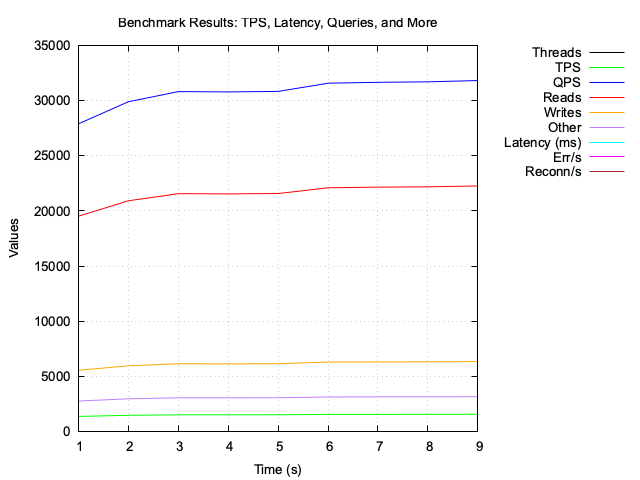
\includegraphics[width=\textwidth]{PNGs/Demo/sysbench_output}
        \label{demo-gnuplot}
    \end{subfigure}
    \hfill
    \begin{subfigure}[t]{0.48\textwidth}
        \centering
        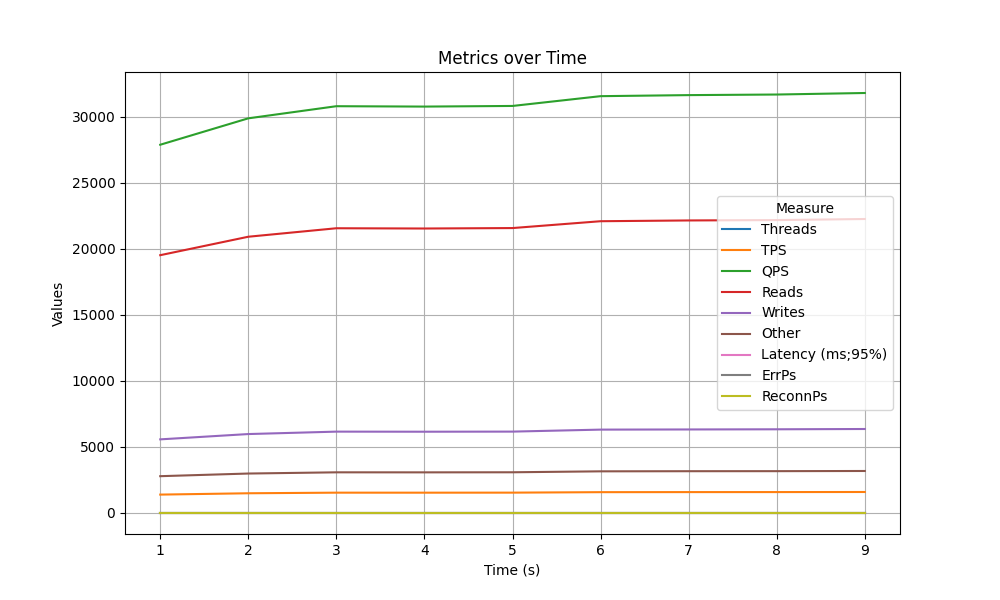
\includegraphics[width=\textwidth]{PNGs/Demo/Summary}
        \label{demo-pandas}
    \end{subfigure}
    \caption[Demo-Graphs: Gnuplot vs. Pandas]{Die Grafik zeigt die erstellten Graphen mit Gnuplot (links) und Pandas (rechts)}
    \label{fig:demo-graph-generation}
\end{figure}


\begin{itemize}
    \item \textbf{Threads}: Die Anzahl der gleichzeitig verwendeten Threads.
    Mehr erhöhen die Parallelität, jedoch zu viele können zur Überlastung des Systems führen.
    \item \textbf{TPS (Transactions Per Second)}: Die Anzahl der Transaktionen pro Sekunde.
    Ein höherer Wert deutet auf eine bessere Datenbankleistung hin.
    \item \textbf{QPS (Queries Per Second)}: Die Anzahl der Abfragen pro Sekunde.
    Ein höherer Wert ist besser und zeigt die Effizienz bei der Verarbeitung von Abfragen.
    \item \textbf{Reads}: Die Anzahl der Leseoperationen.
    \item \textbf{Writes}: Die Anzahl der Schreiboperationen.
    \item \textbf{Other}: Bezieht sich auf andere Arten von Operationen, die weder als Reads noch als Writes kategorisiert werden.
    \item \textbf{Latency (ms; 95\%)}: Die durchschnittliche Zeit in Millisekunden, die benötigt wird, um Anfragen zu bearbeiten, wobei der Wert im 95. Perzentil betrachtet wird.
    Niedrigere Werte sind besser, da sie auf schnellere Reaktionszeiten hinweisen.
    \item \textbf{ErrPs (Errors Per Second)}: Die Anzahl der Fehler pro Sekunde.
    Ein niedriger Wert weist auf höhere Stabilität und Zuverlässigkeit des Systems hin.
    \item \textbf{ReconnPs (Reconnects Per Second)}: Die Anzahl der Wiederverbindungen pro Sekunde.
    Häufige Wiederverbindungen können auch auf Stabilitätsprobleme hindeuten.
\end{itemize}

\section{Genauere Darstellung anhand eines Beispiels}\label{sec:genauere-darstellung-anhand-eines-beispiels}
In dem vorausgegangenen Kapitel \nameref{sec:einfuhrung-in-die-tools} wurde das Tool Sysbench und seine Funktionsweise anhand eines Demo - Projekts näher erläutert.
Damit die Reihenfolge und die Bedeutungen der unterschiedlichen Methoden (prepare → run → cleanup) sowie die Vorgehensweise zur Erstellung unserer Grafiken deutlich geworden.
Das bisherige Problem ist aber, dass wir bei dem dargelegten Beispiel keine Kontrolle über die getesteten Daten haben.
Wenn man sich die Logs genauer anschaut, dann sieht man, dass man über die Parameter an den Sysbench – Befehl die Anzahl der erstellten Tabellen und eingefügten Datensätze von außen steuern kann, aber die genaue Implementierung können wir auf diese Weise nicht steuern.
Genau für diese Anwendungsfälle gibt es die Möglichkeit ein Lua - Skript als Parameter beim Sysbench - Aufruf mit anzugeben.
In diesen Lua - Dateien können die Implementierungen der einzelnen Methoden selbstständig gewählt werden.

Um das Vorgehen besser erklären zu können, schauen wir uns dafür ein Beispiel an.
Für das Beispiel wollen wir zwei Tabellen erstellen und anschließend mit zufälligen Testdaten befüllen.
Die Abfrage, die wir auf Performance testen wollen, ist das Verbinden (Joinen) dieser beiden Tabellen.
In unserem Fall wollen wir eine Kundentabelle erstellen, die Informationen wie Name, Geburtstag und Adresse enthält, sowie eine Bestelltabelle, die Details wie Artikelnummer, Bestelldatum usw. speichert und einen Bezug zu dem Kunden herstellt, der die Bestellung aufgegeben hat.
Damit wir aber nicht nur ein Beispiel haben, das dargestellt wird, brauchen wir einen Vergleich zwischen zwei verschiedenen Implementierungen.
Dieser Unterschied zwischen den beiden Implementierungen besteht darin, dass in der einen Version die Tabelle eine Kundennummer vom Typ \texttt{Int} enthält, während in der anderen keine Kundennummer vorhanden ist.
Stattdessen wird in der Bestelltabelle auf den Namen (Typ \texttt{Varchar}) verwiesen.
Da Verbundoperationen zu den aufwendigsten Operationen gehören, gehen wir davon aus, dass der kleine Typ \texttt{Int} Performancevorteile gegenüber der anderen Version hat.
Dies gilt es nun mit den Benchmarktest genauer zu untersuchen.

Für die Durchführen der Benchmarks beginnen wir zunächst unabhängig von Sysbench und den Lua – Skripten mit der Spezifizierung der Tabellen, die erstellt werden sollen.
Dies müssen wir einmal mit der Kundennummer und einmal mit dem Namen als Fremdschlüssel der Bestelltabelle machen.
Damit müssen insgesamt vier unterschiedliche Create Table - Befehle umgesetzt werden.
So sehen die Create Table für den Fall mit der Kundennummer aus:

\lstinputlisting[
    language=sql,
    caption=Create Table - Befehl für Tabelle Kunden,
    label={lst:create_table_kunde},
    style=custom_daniel,
]{Scripts/Join_Type/01_Create_Table_Kunde.sql}

\lstinputlisting[
    language=sql,
    caption=Create Table - Befehl für Tabelle Bestellung,
    label={lst:create_table_bestellung},
    style=custom_daniel,
]{Scripts/Join_Type/02_Create_Table_Bestellung.sql}

Anschließend müssen wir diese Befehle in \texttt{prepare()} - Funktion miteinbinden.
Dafür müssen wir einfach die Create Table - Befehle an die Datenbank senden.
Wenn wir bestimmte Indexe oder andere Datenbankstrukturen erstellen wollen würden, dann müssten wir dies ebenfalls in dieser Funktion machen.
Dies ist ein Auszug aus der \texttt{Prepare} - Funktion:

\lstinputlisting[
    language={[5.0]Lua},
    caption=Lua - Script für die Erstellung der Tabellen,
    label={lst:prepare_query},
    style=custom_daniel,
]{Scripts/Join_Type/03_Prepare_Query.lua}

Wenn die Datenbank beispielsweise in einer Produktivumgebung läuft, dann wollen wir, dass die Benchmarks möglichst wenig Einfluss aus sie haben.
Damit ist es das Ziel, dass die Datenbank möglichst wieder in ihrem Anfangszustand ist.
Außerdem sollte der Benchmark beliebig oft nacheinander ausgeführt werden können, ohne zu Problemen zu führen.
Wenn wir aber eine Tabelle erstellen und nicht wieder löschen, dann würde im nächsten Durchlauf der Create Table - Befehl scheitern.
Lösen könnte man dies über Klausel „IF NOT EXITS“ bei der Erstellung der Tabelle hinzufügen oder noch es besser ist es die Tabelle am Ende des Benchmarks einfach zu löschen.
Dafür ist die \texttt{cleanup()} – Funktion vorgesehen:

\lstinputlisting[
    language={[5.0]Lua},
    caption=Lua - Script für das Aufräumen,
    label={lst:cleanup_query},
    style=custom_daniel,
]{Scripts/Join_Type/04_CleanUp_Query.lua}

Wichtig ist dabei, dass man keine Schlüsselintegritäten verletzt.
Da in diesem Fall die Tabelle \texttt{BESTELLUNGMITID} eine Referenz auf die Tabelle \texttt{KUNDENMITID} hat, muss zuerst die Bestelltabelle und danach erst die Kundentabelle entfernt werden.

Jetzt haben wir das Gerüst für die eigentlichen Insert - und Select - Befehle geschaffen.
Bei den Insert - Befehlen können wir entweder mit zufälligen Zahlen die Werte generieren oder wir setzen Listen von Namen fest, aus denen zufällig gewählt werden kann.
Da wir jedoch keine Kontrolle über diese zufällig erstellten Werte haben, müssen wir beim Insert - Befehl die Bedingung „Insert Ignore“ hinzufügen, damit doppelte Schlüsselwerte ignoriert werden und keine Fehler verursachen.
Wir müssen hier auch festlegen, wie viele Datensätze für die Kunden erstellt werden und wie viele Bestellungen pro Kunden es geben soll.
Später werden wir noch eine Möglichkeit kennen lernen, um diese Werte von außen zusteuern.
Um sicherzustellen, dass keine Werte in den Tabellen enthalten sind, können wir alle Datensätze aus den Tabellen entfernen, bevor wir sie hinzufügen.
Damit die Performance der Insert – Query auch gemessen wird, ist es wichtig, dass die \texttt{insert()} - Funktion in der \texttt{event()} – Funktion aufgerufen wird.
Sonst kommt es zu diesem Fehler:
\begin{lstlisting}[style=custom_daniel,label={lst:error_withoutevent}]
FATAL: cannot find the event() function in Join.lua
\end{lstlisting}

\lstinputlisting[
    language={[5.0]Lua},
    caption=Lua - Script für das Einfügen von Daten,
    label={lst:insert_query},
    style=custom_daniel,
]{Scripts/Join_Type/05_Insert_Query.lua}

Die letzte Anweisung, die wir noch brauchen, ist die Select - Abfrage.
Hierbei muss man sich Gedanken machen, welche Abfrage benötigt wird, damit die untersuchten Effekte auch tatsächlich auftreten.
In dem Beispiel brauchen wir deswegen einen Join zwischen den beiden Tabellen über den Fremdschlüssel.

\lstinputlisting[
    language={[5.0]Lua},
    caption=Lua - Script für das Abfragen von Daten,
    label={lst:select_query},
    style=custom_daniel,
]{Scripts/Join_Type/06_Select_Query.lua}

Damit haben wir für unseren Vergleich alle vier Operationen genauer definiert und müssen diese 4 Funktionen nur noch leicht anpassen für die Implementierung mit dem Namen als Fremdschlüssel und ohne die Kundennummer in der Kundentabelle.
Daraufhin benötigen wir noch ein Skript, dass die Operationen in der korrekten Reihenfolge ausführt und die Grafiken generiert.
Wichtig dafür ist die folgende Dateienstruktur, die anhand der Int - Verbunds dargestellt wird.

Damit wir die unterschiedlichen Operationen voneinander trennen können, gibt es folgende Dateienstruktur: Es gibt einen Ordner mit einem beliebigen Namen, z.B. \texttt{int\_queries}, in diesem Ordner befinden sich folgende Dateien:
\begin{itemize}\label{files_structure}
    \item \texttt{int\_queries.lua} $\Rightarrow$ enthält die \texttt{prepare()}- und \texttt{cleanup()}-Funktionen
    \item \texttt{int\_queries\_insert.lua} $\Rightarrow$ enthält die \texttt{insert()}-Funktion
    \item \texttt{int\_queries\_select.lua} $\Rightarrow$ enthält die \texttt{select()}-Funktion
\end{itemize}

Analog muss auch ein Ordner für die Varchar - Vergleich erstellt werden.
Als Letztes brauchen wir nur einen Orchestrator, der das korrekte Lua - Skript ausführt, die Ergebnisse in die richtige Log - Datei schreibt und anschließend die CSV - Dateien und die Grafiken erstellt.
Dieser Orchestrator ist das Shell - Skript: \texttt{sysbench\_script.sh}.

Zudem möchten wir unser Beispiel erweitern, da es auch möglich sein soll, unterschiedliche Längen von Varchar hinzuzufügen.
Dadurch könnten wir nicht nur den Performanceunterschied zwischen Int und Varchar feststellen, sondern auch noch den Einfluss der Länge des Verbundoperators für Varchar.
Dazu benötigen wir eine Hilfsfunktion in \texttt{varchar\_queries\_insert.lua}, die einen zufälligen Namen mit der Länge von einer vorgegebenen Zahl erstellt.
Dieser Name ist damit kein natürlicher Name, sondern einfach eine Kombination von zufälligen Buchstaben, aber für unseren Testfall gehen wir diesen Kompromiss ein.
Wenn wir jetzt zwei unterschiedlichen Längen für Varchar testen wollen, dann müssten wir den Varchar - Ordner mit den oben beschriebenen drei Dateien kopieren und nur die Zeile ändern, die die Länge des zufälligen Namens bestimmt.
Dies würde zu extremer Redundanz führen, weshalb man beim Aufruf des Orchestrator - Scripts, Variablen definieren kann, die im Skript selbst exportiert und in der \texttt{varchar\_queries\_insert.lua} - Datei importiert werden können.

Dies ist die Zeile mit der festgelegten Länge:
\begin{lstlisting}[language={[5.0]Lua},label={lst:without_imported_length}]
local length = 10
\end{lstlisting}

Die Zeile mit der importierten Länge:
\begin{lstlisting}[language={[5.0]Lua},label={lst:with_imported_length}]
local length = tonumber(os.getenv("LENGTH"))
\end{lstlisting}

Den Orchestrator - Script ruft man wie folgt auf:
\lstinputlisting[
    language=sh,
    caption=Befehl zum Ausführen des Orchestrator Skripts,
    label={lst:orchestrator_command},
    style=custom_daniel,
]{Scripts/Join_Type/07_Orchestrator_Command.sh}

Die Parameter haben folgende Funktion:
\begin{itemize}[label=--]
    \item \texttt{-out}: Gibt den Pfad an, an welchen der Output-Ordner gespeichert werden soll
    \item \texttt{-var}: Angabe der Variablen und deren Werte, die exportiert werden sollen im JSON-Format
    \item \texttt{-scripts}: Angabe der Pfade zu den Ordnern, die die Lua-Skripte enthalten. Nach dem Doppelpunkt wird angegeben, welche Variable das Skript benötigt. \texttt{Int\_queries} benötigt keine Variablen, deshalb gibt es auch keinen Doppelpunkt.
\end{itemize}

Die letzte Besonderheit ist es, dass man mehrere Select – Abfragen ohne unterschiedliche Insert - Befehle definieren kann.
Zu einem späteren Punkt in der Bachelorarbeit werden wir zu unterschiedliche Indextypen kommen.
Um zu untersuchen, ob ein bestimmter Indextyp bei Abfragen verwendet wird, müssen wir nur unterschiedliche Selects abfragen.
Die eigentlichen Tabellen und deren Datensätze müssen dabei nicht immer wieder gleich befüllt werden.
Wenn wir auch unsere Ordnerstruktur mit dem Int - Query Beispiel zurückkommen, dann könnte man anstelle von \texttt{int\_queries\_select.lua} auch einen Ordner erstellen mit den Namen \texttt{int\_queries\_select}.
In diesem Ordner können beliebig viele unterschiedliche Lua - Skripts sein, die select – Funktionen haben.
Dadurch werden alle Select - Befehle auf der gleichen Datenbasis verglichen und so können wir im Kapitel (TODO (Daniel): Index) erkennen, wann der Index verwendet wird und wann nicht.

Bevor wir uns das Ergebnis des Befehls anschauen, kommen wir zu der Funktionsweise des Orchestrator - Skript \texttt{sysbench\_script.sh}.
Im Grundlegenden arbeitet dieses Skript ähnlich wie schon das Skript im Demo - Beispiel, aber durch die zusätzlichen Anwendungsfälle kommt es zu mehr Komplexität.

Zu Beginn des Skripts werden die Umgebungsvariablen aus der Datei \texttt{db.env} geladen.
Die Variablen helfen zum einen wie bei dem Demo - Beispiel bei die Datenbank - Verbindung und zum anderen können sich auch die Parameter der Benchmarks verändern.
Danach werden die Parameter, die an das Skript übergeben wurden, überprüft.
Beispielsweise wird sichergegangen, dass die für die Skripts verwendeten Parameter, bei unserem Beispiel length für varchar, tatsächlich auch definiert worden sind mit \texttt{-var}.

Wenn wir den Befehl ausführen, wird der Output-Ordner an der gewünschten Stelle erstellt.
In diesem Ordner werden verschiedene Grafiken generiert, die die Ergebnisse visualisieren.
Dabei gibt es zwei unterschiedliche Arten von Grafiken.
Die erste Art von Grafik ist ein Zeitreihendiagramm, welches auf der x-Achse den zeitlichen Verlauf zeigt.
Auf der y-Achse werden in einigen Diagrammen die unterschiedlichen Metriken für jedes einzelne Skript dargestellt, während andere Diagramme die Werte einer bestimmten Metrik auf der y-Achse zeigen und dabei die Ergebnisse verschiedener Skripte vergleichen.
Dadurch können beispielsweise die Metriken \texttt{Reads} und \texttt{Writes} analysiert werden, um herauszufinden, welches Skript in diesen Bereichen besser abschneidet.
Danach wird der Output - Ordner erstellt und die Spaltenüberschriften in die CSV – Dateien geschrieben.
Danach beginnt erst das eigentliche Durchgehen der unterschiedlichen Skripte, die unter dem Argument -script angegeben wurden.
Zunächst schreibt man die einzelnen Dateien nach dem obigen Schema (\ref{files_structure}) auf, denn als Argument wurde nur der oberste Ordner angegeben.
Als nächstes kommt eine Fallunterscheidung, die überprüft, ob dieses Skript exportierte Variable nutzt oder nicht.
Für den Fall, dass keine Variablen exportiert werden (z.B. \texttt{int\_queries}) wird einfach die Prepare – Funktion aufgerufen, dann \texttt{process\_script\_benchmark} und anschließend die Cleanup - Funktion.
Wenn aber Variablen exportiert werden, dann müssen weitere Zwischenschritte umgesetzt werden.
Und zwar müssen alle Kombinationen zwischen den verschiedenen exportierten Variablen generiert werden.
Wenn es drei Variablen gibt, von denen 2 jeweils 2 Werte und eine letzte nur einen Wert hat, dann gibt es 2 * 2 * 1 = 4 unterschiedliche Kombinationen.
Als nächstes muss man für alle diese Kombinationen die Schritte ausführen, die man schon bei der Variante ohne exportierte Variable ausgeführt hat und dabei darf man nicht vergessen die Variablen an sich zu exportieren.

\lstinputlisting[
    language=sh,
    caption=Ausschnitt aus Orchestrator Script,
    label={lst:main_loop},
    style=custom_daniel,
]{Scripts/Join_Type/08_Main_Loop.sh}

Die Funktion \texttt{process\_script\_benchmark} überprüft noch es sich bei dem Select – Directory um einen Ordner handelt oder nicht.
Wenn es ein Ordner ist, dann werden alle Dateien in diesem Ordner mit Sysbench durchgeführt, wenn nicht, dann wird an den Ordner nur die Endung \texttt{.lua} hinzugefügt.

\lstinputlisting[
    language=sh,
    caption=Methode Process Script Benchmark,
    label={lst:process_script_benchmark},
    style=custom_daniel,
]{Scripts/Join_Type/09_Process_Script_Benchmark.sh}

Die Methode \texttt{run\_benchmark} führt den Sysbench – Befehl aus und wenn es sich um die Methode \texttt{Run} handelt, dann müssen die Daten während der Ausführung und die Statistiken am Ende in je eine CSV - Datei speichern.
Aus diesen beiden CSV - Dateien müssen die Insert - und Select - Queries der zugehörigen Skripte wieder vereint werden und die Attribute werden miteinander addiert.
Als letzter Schritt erfolgt noch der bekannte Schritt der Grapherstellung.

\lstinputlisting[
    language=sh,
    caption=Methode Run Benchmark,
    label={lst:run_benchmark},
    style=custom_daniel,
]{Scripts/Join_Type/10_Run_Benchmark.sh}

INFO: Die Shell - Ausschnitte sind zum Teil verkürzt und würden auf diese Weise nicht funktionieren.

Wenn wir den Befehl ausführen, wird der Output-Ordner an der gewünschten Stelle erstellt.
In diesem Ordner werden verschiedene Grafiken generiert, die die Ergebnisse visualisieren.
Die erste Art stellen Zeitreihendiagramme dar, die auf der X-Achse den zeitlichen Verlauf zeigen.
Auf der Y-Achse werden hingegen in einigen Diagrammen die unterschiedlichen Metriken eines einzelnen Skripts dargestellt, während andere Diagramme die Werte einer bestimmten Metrik auf der Y-Achse zeigen und dabei die Ergebnisse verschiedener Skripte vergleichen.
Dadurch können beispielsweise die Metriken "Reads" und "Writes" analysiert werden, um herauszufinden, welches Skript in diesen Bereichen besser abschneidet.

Die zweite Art von Grafik, die erstellt wird, ist ein Hexagon - Diagramm.
Dieses verzichtet auf eine Zeitachse und fasst die Performance über den gesamten Zeitraum hinweg zusammen.
Im Vergleich zur Laufzeitanalyse liefert es zusätzliche Informationen, wie etwa die Latenz oder die Gesamtanzahl der Queries.
Dadurch ist es auch möglich, dass mehrere Skripte und mehrere Kennzahlen in einer Grafik dargestellt werden können.

PNGs

\begin{figure}[!ht]
    \centering
    \begin{subfigure}[t]{0.48\textwidth}
        \centering
        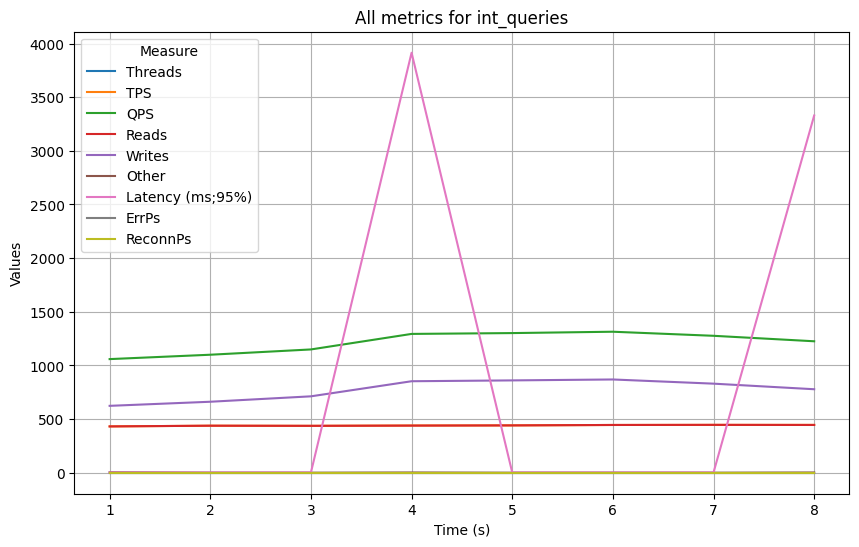
\includegraphics[width=\textwidth]{Scripts/Join_Type/PNGs/int_queries}
        \label{join-typ-int_queries}
    \end{subfigure}
    \hfill
    \begin{subfigure}[t]{0.48\textwidth}
        \centering
        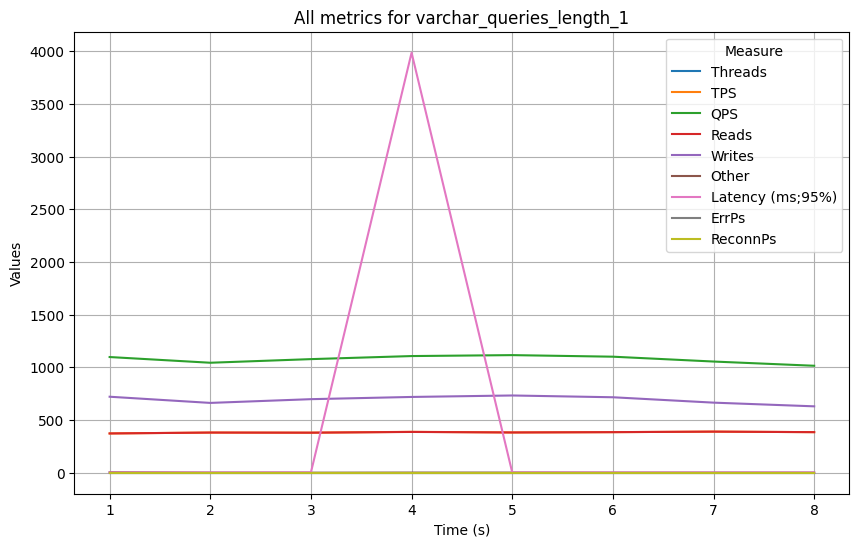
\includegraphics[width=\textwidth]{Scripts/Join_Type/PNGs/varchar_queries_length_1}
        \label{join-typ-varchar_queries_length_1}
    \end{subfigure}
    \caption[Join-Typ: Skriptvergleich]{Die Grafik zeigt alle Metriken für die Skripte \texttt{int\_queries} (links) und \texttt{varchar\_queries\_length\_1} (rechts)}
    \label{fig:join-typ-comp-script}
\end{figure}

\begin{figure}[!ht]
    \centering
    \begin{subfigure}[t]{0.48\textwidth}
        \centering
        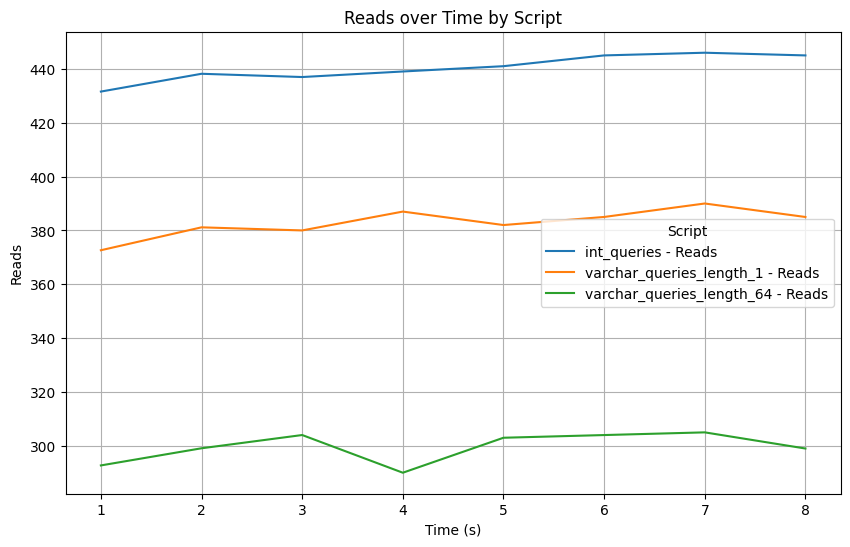
\includegraphics[width=\textwidth]{Scripts/Join_Type/PNGs/Reads}
        \label{join-typ-reads}
    \end{subfigure}
    \hfill
    \begin{subfigure}[t]{0.48\textwidth}
        \centering
        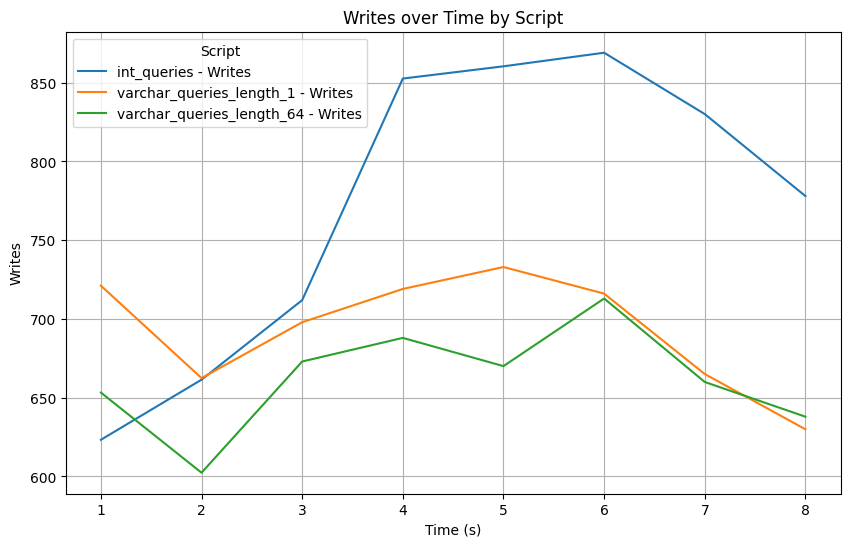
\includegraphics[width=\textwidth]{Scripts/Join_Type/PNGs/Writes}
        \label{join-typ-writes}
    \end{subfigure}
    \caption[Join-Typ: Metrikvergleich]{Die Grafik zeigt den Vergleich zwischen allen Skripten für die Metriken Reads (links) und Writes (rechts)}
    \label{fig:join-typ-comp-metric}
\end{figure}

\begin{figure}[!ht]
    \centering
    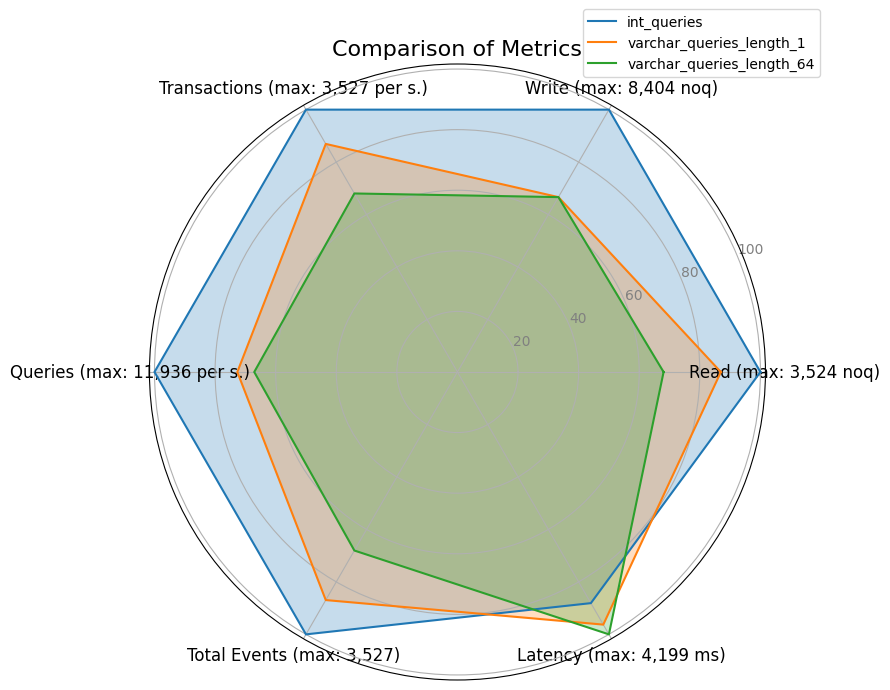
\includegraphics[width=.7\textwidth]{Scripts/Join_Type/PNGs/statistics}
    \caption[Join-Typ: Hexagon-Diagramm]{Darstellung der Skripte und 6 Metriken in einem Hexagon}
    \label{fig:join-typ-hex}
\end{figure}

Aus den Grafiken, die für ein Skript alle Metriken veranschaulichen, kann man möglicherweise Datenfehler erkennen.
So springt bei Abbildung (\texttt{int\_queries.png}) die Latenz bei einigen Messpunkten von 0 ms auf einen deutlich erhöhten Wert und danach wieder auf 0 ms zurück.
Ansonsten aber sind die anderen Metriken auf einem konstanten Level, und es gibt wenige Schwankungen.
Bei der Abbildung (\texttt{varchar\_queries\_length\_1.png}) sieht dies sehr ähnlich aus, und auch dort schwankt die Latenz etwas mehr.
Wenn wir jetzt die drei Skripte miteinander vergleichen wollen, können wir die Abbildungen Reads.png und Writes.png heranziehen.
Was die Lesegeschwindigkeit angeht, kann man erkennen, dass \texttt{int\_queries} am meisten Reads hat, als Nächstes kommt \texttt{varchar\_queries\_length\_1} und dann \texttt{varchar\_queries\_length\_64}.
Damit sind die Abfragen, wie wir erwartet haben, bei \texttt{int\_queries} am schnellsten, und je länger der String wird, desto langsamer werden die Abfragen.
Bei den Schreibgeschwindigkeiten sieht das schon etwas anders aus, wobei es hier zunächst bei allen eine langsamere Startphase gibt.
Anschließend an diesen Cold Start liegt das Niveau von \texttt{int\_queries} am höchsten, also auch am schnellsten.
Die beiden \texttt{varchar\_queries} sind hier aber überraschenderweise auf einem ähnlichen Niveau.
Bei der Abbildung (\texttt{statistics.png}) kann man die Effekte der Lese- und Schreibgeschwindigkeiten auch erkennen.
Es fällt auch auf, dass, anders als bei Reads, Writes, Queries, die Latenz bei schnelleren Queries geringer ist und nicht der höchste Wert der Beste ist.